\chapter{Conclusión}  \label{conclusion_sec}

\section{Características del proyecto}
\begin{itemize}
\item Implementación de la operación de convolución bidimensional en una FPGA
\item Particionamiento de imagen por columnas, y carga de las mismas en la placa
\item Manejo de uno o más módulos convolucionadores y memorias, es decir, procesamiento con cierto grado de paralelismo
\item Kernel de $ k \times k$, con $k$ configurable
\item Manejo de imágenes de escala de grises (cada píxel tiene asociado un valor de intensidad ó escala de gris)
\item Reutilización de hardware mediante un algoritmo descubierto y llevado a cabo en la implementación
\item Funcionalidades y etapas en su totalidad: el sistema implementado cubre todas las etapas (carga, procesamiento, devolución)
\item Escalabilidad
\end{itemize}
    
La flexibilidad y elevada potencia de cálculo de una FPGA permite que se pueda
procesar y filtrar el lote de imagen, al mismo tiempo que se está cargando el lote
actual.

Se diseñó y presentó una implementación de la operación de convolución
bidimensional en una plataforma Xilinx Artix 7 FPGA basada en eficiencia en la
utilización de recursos y en el paralelismo del sistema.

Se implementaron todas las etapas necesarias, considerando la etapa de carga,
procesamiento, y salida.

Se encontró una relación entre ciertos bloques
instanciados, lo que permitió a nuestro sistema trabajar con diferentes niveles
de paralelismo.

Ademas, se optimizó la utilización de recursos de almacenamiento implementando
un algoritmo para las operaciones con memoria y para la sincronización de
módulos. Esto permitió con una parametrización total del sistema, lo que hace
escalable a la arquitectura propuesta.

El desempeño del sistema y los resultados obtenidos muestran que la utilización
de recursos relacionados con Block RAMs incrementan de forma lineal, como se
esperaba. 

En lo que refiere al procesamiento, se obtuvo un throughput elevado, por ende
del factor limitante mencionado relacionado con la velocidad de transmisión del
UART.

\section{Futuras mejoras}
Se plantean como mejoras posibles, la carga de la imagen completa, de disponer una FPGA más grande y tener un medio de comunicación más rápido (Ethernet , por ejemplo) 
ya que más de un 99$\%$ del tiempo el sistema lo invierte en la carga. El procesamiento es muy rápido en relación al tiempo invertido en la carga de datos.
Otras posibles mejoras incluirian trabajar con menos bits en lo que refiere a la resolución de la salida (actualmente 13 bits),  y el aprovechamiento del bus del GPIO para cargar 3 memorias por escritura en la etapa 
de carga correspondiente. (Actualmente, por escritura se carga una sola). Análogamente para la etapa de salida de datos.
De ser el tamaño de la imagen menor a la profundidad de las memorias definidas, se desaprovechan los restantes registros. 
Una última  futura mejora también sería el aprovechamiento total de las mismas en dicha situación

\section{Publicación en CASE-2018}
Ademas del tiempo invertido en el desarrollo del trabajo a fines de realizar la
Practica Profesional Supervisada, se logró publicarlo en el Congreso Argentino
de Sistemas Embebidos del año actual. Dicha publicación fue una gran experiencia
que sirvió para adquirir conocimientos y práctica sobre como elaborar artículos
técnicos y científicos.

\begin{figure}
\centering
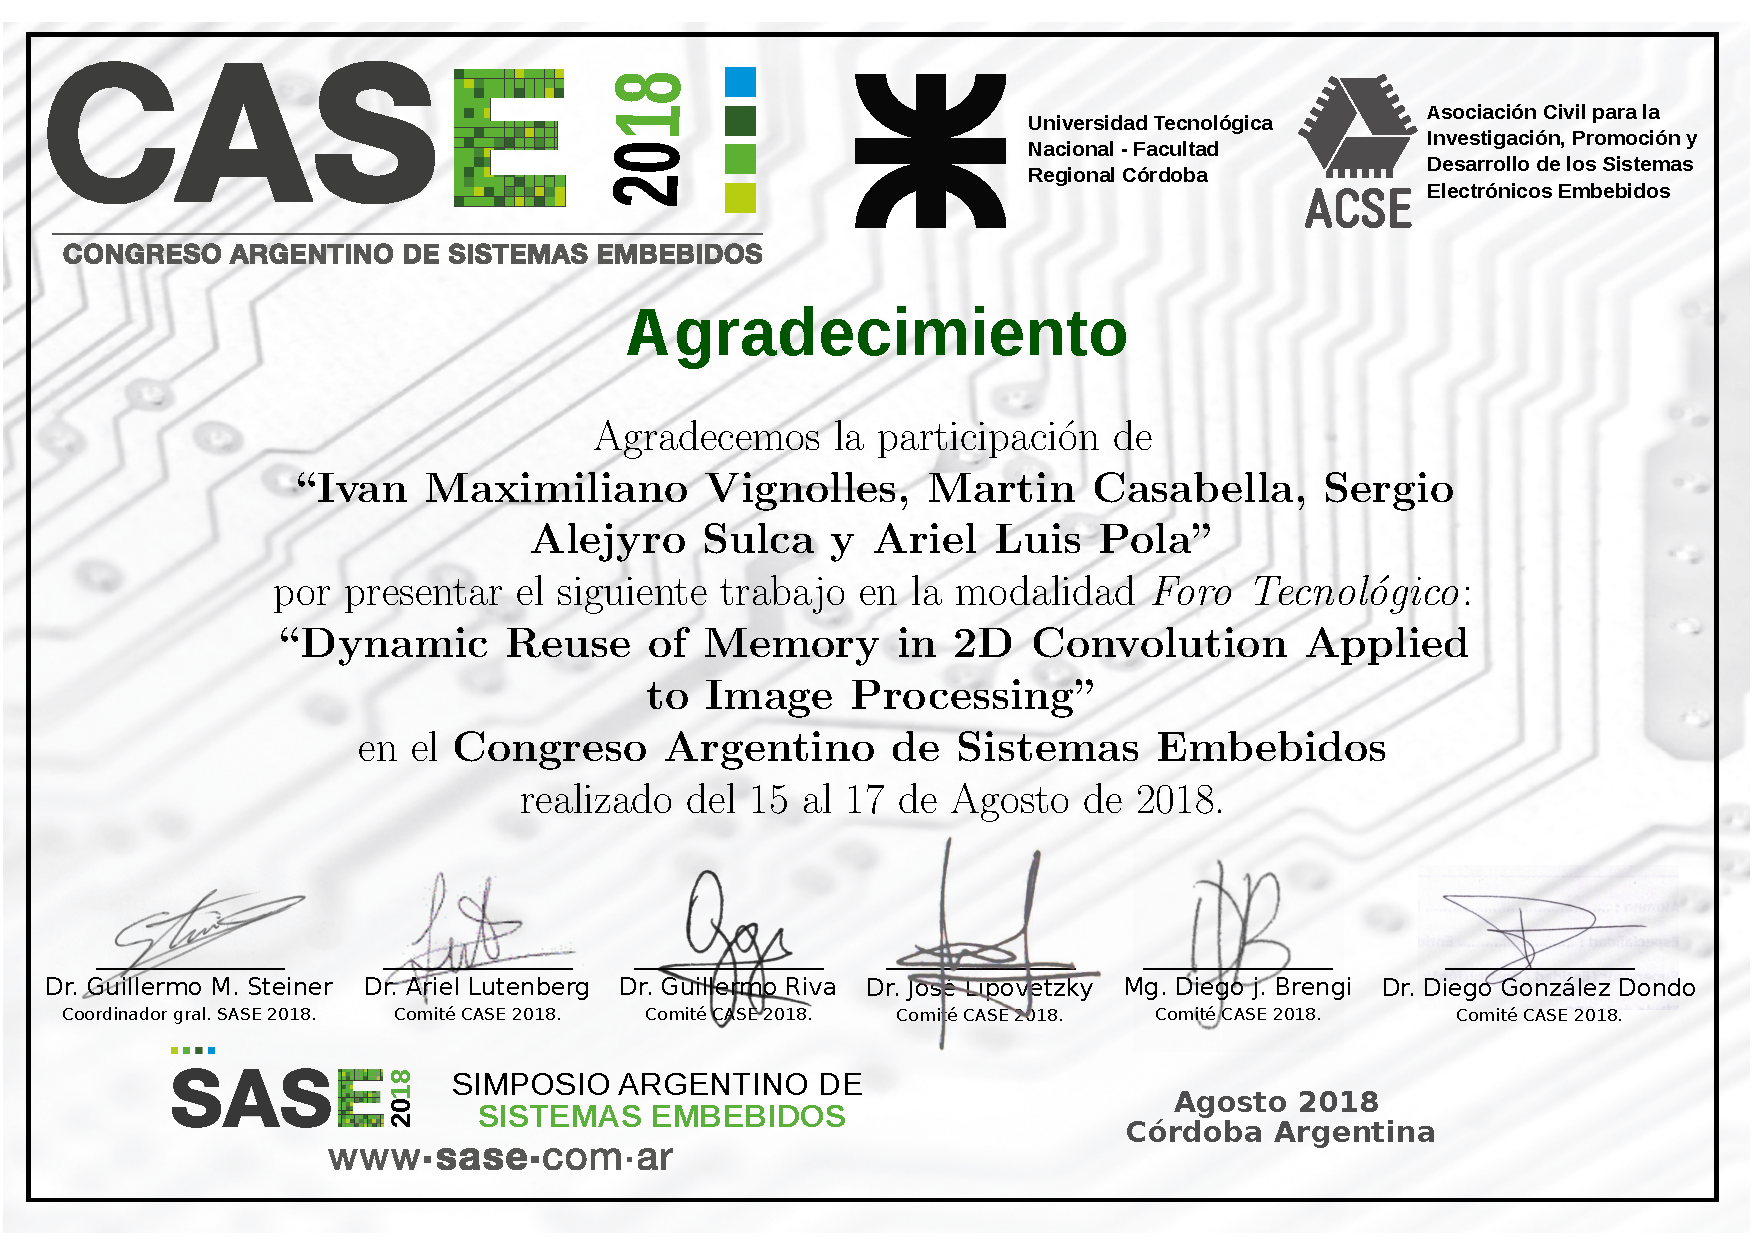
\includegraphics[scale=0.5]{certificado_CASE}
\caption{Certificado por la publicación del proyecto llevado a cabo.}
\label{CASE}
\end{figure}